%% This is file `elsarticle-template-1-num.tex',
%%
%% Copyright 2009 Elsevier Ltd
%%
%% This file is part of the 'Elsarticle Bundle'.
%% ---------------------------------------------
%%
%% It may be distributed under the conditions of the LaTeX Project Public
%% License, either version 1.2 of this license or (at your option) any
%% later version.  The latest version of this license is in
%%    http://www.latex-project.org/lppl.txt
%% and version 1.2 or later is part of all distributions of LaTeX
%% version 1999/12/01 or later.
%%
%% The list of all files belonging to the 'Elsarticle Bundle' is
%% given in the file `manifest.txt'.
%%
%% Template article for Elsevier's document class `elsarticle'
%% with numbered style bibliographic references
%%
%% $Id: elsarticle-template-1-num.tex 149 2009-10-08 05:01:15Z rishi $
%% $URL: http://lenova.river-valley.com/svn/elsbst/trunk/elsarticle-template-1-num.tex $
%%
\documentclass[preprint,12pt]{elsarticle}

%% Use the option review to obtain double line spacing
%% \documentclass[preprint,review,12pt]{elsarticle}

%% Use the options 1p,twocolumn; 3p; 3p,twocolumn; 5p; or 5p,twocolumn
%% for a journal layout:
%% \documentclass[final,1p,times]{elsarticle}
%% \documentclass[final,1p,times,twocolumn]{elsarticle}
%% \documentclass[final,3p,times]{elsarticle}
%% \documentclass[final,3p,times,twocolumn]{elsarticle}
%% \documentclass[final,5p,times]{elsarticle}
%% \documentclass[final,5p,times,twocolumn]{elsarticle}

%% if you use PostScript figures in your article
%% use the graphics package for simple commands
%% \usepackage{graphics}
%% or use the graphicx package for more complicated commands
\usepackage{graphicx}
%% or use the epsfig package if you prefer to use the old commands
%% \usepackage{epsfig}

%% The amssymb package provides various useful mathematical symbols
\usepackage{amsmath,amssymb}
\usepackage{bm}
%\usepackage[numbers,sort&compress]{natbib}
\usepackage{color}
\usepackage{tabularx}

%% The amsthm package provides extended theorem environments
%% \usepackage{amsthm}

%% The lineno packages adds line numbers. Start line numbering with
%% \begin{linenumbers}, end it with \end{linenumbers}. Or switch it on
%% for the whole article with \linenumbers after \end{frontmatter}.
\usepackage{lineno}

%% natbib.sty is loaded by default. However, natbib options can be
%% provided with \biboptions{...} command. Following options are
%% valid:

%%   round  -  round parentheses are used (default)
%%   square -  square brackets are used   [option]
%%   curly  -  curly braces are used      {option}
%%   angle  -  angle brackets are used    <option>
%%   semicolon  -  multiple citations separated by semi-colon
%%   colon  - same as semicolon, an earlier confusion
%%   comma  -  separated by comma
%%   numbers-  selects numerical citations
%%   super  -  numerical citations as superscripts
%%   sort   -  sorts multiple citations according to order in ref. list
%%   sort&compress   -  like sort, but also compresses numerical citations
%%   compress - compresses without sorting
%%
%% \biboptions{comma,round}

% \biboptions{}

\journal{Chemical Engineering Journal}

\newcommand{\Ca}{\mathrm{Ca}}
\newcommand{\todo}[1]{{\color{red}#1}}

\begin{document}

\begin{frontmatter}
%% Title, authors and addresses

%% use the tnoteref command within \title for footnotes;
%% use the tnotetext command for the associated footnote;
%% use the fnref command within \author or \address for footnotes;
%% use the fntext command for the associated footnote;
%% use the corref command within \author for corresponding author footnotes;
%% use the cortext command for the associated footnote;
%% use the ead command for the email address,
%% and the form \ead[url] for the home page:
%%
%% \title{Title\tnoteref{label1}}
%% \tnotetext[label1]{}
%% \author{Name\corref{cor1}\fnref{label2}}
%% \ead{email address}
%% \ead[url]{home page}
%% \fntext[label2]{}
%% \cortext[cor1]{}
%% \address{Address\fnref{label3}}
%% \fntext[label3]{}

\title{The binary liquid model for gravity-driven microchannel simulations}

%% use optional labels to link authors explicitly to addresses:
%% \author[label1,label2]{<author name>}
%% \address[label1]{<address>}
%% \address[label2]{<address>}

\author[uofa]{A.~Kuzmin\corref{cor1}}
\cortext[cor1]{Corresponding author}
\ead{shurik.kuzmin@gmail.com}
\author[us]{M.~Januszewski}
\ead{michalj@gmail.com}
\author[uofa]{J.~Derksen}
\ead{kuzmin@ualberta.ca}
\author[schlum]{D.~Eskin}
\ead{deskin@slb.com}
\author[schlum]{F.~Mostowfi}
\ead{fmostowfi@slb.com}
\address[us]{Insitute of Physics, University of Silesia, 40-007 Katowice, Poland}
\address[uofa]{Chemical and Materials Engineering, University of Alberta\\ 7th Floor, ECERF, 9107
116 St, Edmonton, Alberta, T6G
2V4 Canada}
\address[schlum]{DBR Schlumberger Technology Center\\ 9450 17 Ave NW, Edmonton, Alberta, T6N 1M9
Canada}

\begin{abstract}
This work shows that the free-energy binary liquid lattice Boltzmann method is able to
reproduce the gravity driven microchannel flow of a gas bubble through liquid. In the regime of low
capillary
numbers
$\Ca$ (defined in Eq.~\ref{capillary:number:definition}), the flow is thoroughly described by
Bretherton \cite{bretherton},
with the deposition film thickness proportional to $\Ca^{2/3}$. However, there are deviations
from the Bretherton correlation for $\Ca\geq 0.005$, studied experimentally and numerically. This
work aims to examine the applicability of the lattice Boltzmann binary liquid model to simulations
of bubble flow in liquids for a range of $\Ca$ numbers. The binary
liquid model is a continuous-interface multiphase model allowing to properly resolve the interface.
It was found that the interface thickness needs to be $50$
percent of the film thickness for the simulation to give convergent results. When
the convergence criterion is fulfilled, the results are in a good agreement with the
numerical simulations of \citet{giavedoni-numerical} in the range of $\Ca$ from $0.01$ to $1$. 
\end{abstract}

\begin{keyword}
Bretherton problem \sep Microchannel simulation \sep Multiphase flow \sep Lattice Boltzmann method
\sep Binary liquid model \sep Flow between plates \sep Gravity driven
%% keywords here, in the form: keyword \sep keyword

%% MSC codes here, in the form: \MSC code \sep code
%% or \MSC[2008] code \sep code (2000 is the default)
\end{keyword}

\end{frontmatter}

%%
%% Start line numbering here if you want
%%
\linenumbers

%% main text

%% The Appendices part is started with the command \appendix;
%% appendix sections are then done as normal sections
%% \appendix

%% \section{}
%% \label{}

%% References
%%
%% Following citation commands can be used in the body text:
%% Usage of \cite is as follows:
%%   \cite{key}          ==>>  [#]
%%   \cite[chap. 2]{key} ==>>  [#, chap. 2]
%%   \citet{key}         ==>>  Author [#]

\section{Introduction}
The Taylor/Bretherton \cite{bretherton} flow describes the flow of long bubbles in
microchannels. It was found that the front meniscus film thickness is proportional
to $\Ca^{2/3}$ for capillary numbers smaller than $0.003$, where the capillary number is defined as:
\begin{equation}
\label{capillary:number:definition}
\Ca=\frac{\mu_\mathrm{liq} U_\mathrm{bubble}}{\gamma},
\end{equation}
where $\mu_{liq}$ is the liquid viscosity, $U_{bubble}$ is the bubble velocity, and
$\gamma$ is the surface tension between gas and liquid.

While there are a number
of works which simulate the Bretherton problem by the boundary value approach
\cite{ingham-plates,heil-bretherton}, those methods are of limited applicability for problems
involving complex geometries, free interface motion, or for problems involving coalescence and/or
droplet breakup. The continuous interface models are more flexible for those kind of simulations.
However, if the interface is spread over several grid nodes, the question of
proper film resolution in comparison with the interface resolution arises.  This work is focused on
resolving the parameter range of the binary liquid lattice
Boltzmann method to validate it for a range of capillary numbers.

The lattice Boltzmann method has emerged as a successful method to simulate
a wide variety of phenomena including hydrodynamics \cite{yu}, thermal flows
\cite{karlin-minimalmodels}, microflows \cite{ansumali-small-knudsen},
ferrofluids \cite{kuzmin-aniso}, and multiphase flows
\cite{swift,Shan-chen:extended}. Thanks to its kinetic nature, LBM as a particle
method easily tackles complex geometries and allows incorporation of
physical phenomena on the microscopic level, as in the case of multiphase models. Most
multiphase lattice Boltzmann models \cite{swift, Shan-chen:extended} resolve
the interface using continuous interface methods where the interface spans over several grid nodes.
Such a representation
brings issues of the film thickness resolution versus interface
resolution -- the diffuse interface should be resolved in such a way as to have
negligible effect on the physics of the film.

The binary liquid free-energy LB model \cite{swift} we used
simulates two liquids with the assumption of uniform overall
density. While the classical Bretherton problem is stated for gas and liquid, which are of
significantly
different densities and viscosities, it was indicated \cite{bretherton} that inertia effects were
neglected. Moreover, the results of \citet{giavedoni-numerical} and \citet{heil-bretherton} show
negligible Reynolds number effect on the film thickness for a relatively wide range of Reynolds
numbers.
Therefore, the major governing factor for microchannel flows is not the density ratio, but the
viscosity ratio. Moreover, the results based on the uniform density, as in the case of the LBM
binary liquid model, are in good agreement with other simulations
\cite{giavedoni-numerical,heil-bretherton} in which inertia effects were taken into account.

The goal of this paper is to understand how to choose the
binary liquid model parameters, the viscosity ratio and the grid
resolution to obtain correct film thicknesses.

The paper is organized as follows.  First, we briefly
explain the binary liquid lattice Boltzmann model and review the literature
for the Bretherton problem. Then, the parameters involved in the
simulation are examined and presented in the results section. The paper is
concluded with a summary of the main findings.

\section{Bretherton bubble flow}
Bretherton \cite{bretherton} studied a long bubble
moving in a tube filled with liquid. It was found that the deposition film thickness
is proportional to $\Ca^{2/3}$ in the range of small capillary numbers. Later on
it was realized \cite{wong-films,wong-pressure} that the film thickness
is proportional to $\Ca^{2/3}$ only in the certain region behind the front meniscus and
that the film thickness
varies over the bubble length for bubbles of finite length. Numerical
simulations \cite{giavedoni-numerical} and experimental studies
\cite{kreutzer-pressure-drop} showed a deviation from the $\Ca^{2/3}$ rule and Reynolds number 
effect on the film thickness for capillary numbers larger than $0.003$.
To  predict consistently a flow pattern for capillaries in
different ranges of parameters, simulations have been conducted and have been typically validated with the
small capillary numbers Bretherton problem.

There are a number of numerical methods which
were used for the simulation of the Taylor/Bretherton flow.
\citet{vanbaten-circular} studied the mass transfer and film
thickness for rising bubbles in a circular capillary using the finite volume method.
\citet{kreutzer-pressure-drop} also used the finite volume method to perform
simulations of a circular capillary for a number of different
Reynolds and capillary numbers. \citeauthor{wong-films} \cite{wong-films,wong-pressure} studied
three-dimensional bubbles in
polygonal capillaries and showed calculated different shapes in the
slug cross sections and menisci appearance.
\citet{heil-bretherton,ingham-plates} studied gas finger propagation in
a two-dimensional channel for a range of Reynolds and capillary
numbers using the finite element method. \citet{giavedoni-numerical} performed cross validation of the
finite element solution with previously published results.
The solutions were obtained for circular and planar cases.

While the applicability of other methods has been demonstrated for the
simulation of the Bretherton/Taylor problem, this is not the case for
the lattice Boltzmann method. A thorough parametric study for this approach
has not been done to the best of the authors' knowledge.

One should acknowledge the works of \citet{pagonabarraga-fingers} on menisci
in thin films for fingering phenomena. \citet{sehgal-microchannel} performed lattice Boltzmann
simulations of two-dimensional channel flows for a relatively large capillary numbers, and
the authors found discrepancies with the classical Bretherton theory, which
is limited to the low capillary number regime \cite{giavedoni-numerical}.

Resolving the interface on a fine level for capillary numbers smaller than
$0.003$ is computationally expensive even in the two-dimensional case
(the amount of memory necessary to perform the simulation is of the order
of tens or hundreds gigabytes).  This work is therefore based on a
comparison of the results obtained with the known data
validated for the Bretherton bubble flow.  In this paper, we present
techniques for initialization of the simulations and discuss optimal
parameter ranges for the binary liquid LB model.

\section{Lattice Boltzmann binary liquid model}
The lattice Boltzmann equation (LBE) operates on a rectangular grid representing the
physical domain. It utilizes
probability distribution functions (also known as particle populations)
containing information about
macroscopic variables, such as fluid density and momentum. LBE consists of
two parts: a local collision step, and a propagation step which transports
information from one node to another in certain
directions specified by the discrete velocity set.
The LBE is typically implemented as follows:
\begin{equation}
\label{standard:implementation}
\begin{aligned}
&f_i^{*}(\bm{x},t)=\omega f_i^{eq}(\bm{x},t)-(1-\omega) f_i(\bm{x},t) +
F_i,&&\text{ collision step}\\
&f_i(\bm{x}+\bm{c_i},t+1)=f_i^{*}(\bm{x},t),&&\text{ propagation step}, 
\end{aligned}
\end{equation}
where $f_i$ is the probability distribution function in the direction $\bm{c_i}$, $\omega$ is the
relaxation parameter, and $F_i$ is the external force population. 

The binary fluid LB model is
based on a free-energy functional \cite{swift,landau}, and operates with two
sets of populations: one to track the pressure and the velocity fields, and another to represent the
phase field $\phi$ indicating the gas or liquid.

The model we use is a two-dimensional nine-velocity (D2Q9) model,
with equilibrium populations \cite{pooley-contact}:
\begin{equation}
\label{set:equilibrium:binary}
\begin{aligned}
&f_i^{eq}&&=w_i 
\biggl(3
p_0 - k \phi \Delta \phi
+\frac{u_{\alpha}c_{i\alpha}}{c_s^2}+\frac{Q_{i\alpha\beta}u_{\alpha } u_ {
\beta}}{2 c_s^4}\biggr)\\
&&&+k\bigl(w_i^{xx} (\partial_x \phi)^2+w_i^{yy} (\partial_y \phi)^2 +w_i^{xy} \partial_x
\phi \partial_y \phi \bigr), i=1\div8\\
&f_0^{eq}&&=\rho-\sum_{i\neq0}{f_i^{eq}}\\
&g_i^{eq}&&=w_i\left(\Gamma \mu + \frac{\phi c_{i\alpha} u_{i\alpha}}{c_s^2}+\phi^m
\frac{Q_{i\alpha\beta}u_{\alpha}u_{\beta}}{2 c_s^4}\right), i=1\div8 \\
&g_0^{eq}&&=\phi-\sum_{i\neq0}{g_i^{eq}}\quad,
\end{aligned}
\end{equation}
where $\Gamma$ is the mobility parameter; the chemical potential
$\mu=-A\phi+A\phi^3-k\Delta\phi$; $k$ is the parameter related to the surface
tension; $A$ is the parameter of the free-energy model.  The bulk pressure
is expressed as $p_0=c_s^2 \rho +A (-0.5 \phi^2+0.75 \phi^4)$. 
Parameters specific to the D2Q9 grid are the weights
$w_i=\left\{\frac{4}{9},\frac{1}{9},\frac{1}{9},\frac{1}{9},\frac{1}{9},
\frac{1}{36},\frac{1}{36},\frac{1}{36},\frac{1}{36}\right\}$, and the tensor
$Q_{i\alpha\beta}=c_{i\alpha} c_{i\beta} - c_s^2 \delta_{\alpha\beta}$ with
the sound speed parameter $c_s^2=1/3$.  The weights related to the
inclusion of the surface tension coefficient into the equations are as follows:
$w^{xx}_{1-2}=w^{yy}_{3-4}=1/3$, $w^{xx}_{3-4}=w^{yy}_{1-2}=-1/6$,
$w^{xx}_{5-8}=w^{yy}_{5-8}=-1/24$, $w^{xy}_{1-4}=0$, $w^{xy}_{5-6}=1/4$ and
$w^{xy}_{7-8}=-1/4$. The set of equations (\ref{set:equilibrium:binary}) restores the
macroscopic
fluid equations as:
\begin{equation}
\begin{aligned}
&\partial_t \rho+ \partial_{\alpha} \rho u_{\alpha}=0\\
&\rho\left(\partial_t+u_{\beta}\partial_{\beta}\right) u_{\alpha}=
-\partial_{\alpha}P_{\alpha \beta} +
\nu\partial_{\beta}\left(\partial_{\alpha}u_{\beta}+\partial_{\beta} u_{\alpha}\right)\\
&\partial_t \phi + \partial_{\alpha} \phi u_{\alpha}=M \partial^2_{\beta\beta} \mu,
\end{aligned}
\label{binary:fluid:system}
\end{equation}
where $\nu=c_s^2 (\tau-1/2)$ is the viscosity and
$M=\Gamma(\tau_{\phi}-1/2)$ is the mobility parameter. 

The system allows the separation of the liquid
phase with $\phi=1$ and a so-called gas phase with $\phi=-1$. The
relaxation time is taken as linearly dependent on the relaxation
times $\tau_{\mathrm{gas}}$ and $\tau_{\mathrm{liq}}$:
$\tau=\tau_{\mathrm{gas}}+\frac{\phi+1}{2}\tau_{\mathrm{liq}}$.
The surface tension in the framework of the binary liquid model is $\sqrt{\frac{8 k A}{9}}$.

\section{Lattice Boltzmann benchmark}
To properly simulate and compare simulation results with the data
published in the literature, one needs to design a numerical benchmark addressing
the following challenges for the lattice Boltzmann method:
\begin{itemize}
 \item The diffuse nature of the interface in the multiphase model should not
influence the film thickness results. This is obviously achieved only for certain
interface resolutions relative to the film thickness. The same applies to spurious
currents arising due to surface tension discretization, which
can influence mass transfer in the thin film, thereby compromising the
overall solution. Therefore, the diffuse interface should not noticeably affect the film
thickness.
 \item The wettability coefficient which in principle can control the
dynamic angle and the menisci appearance \cite{pagonabarraga-finger} should not
influence the overall solution.
 \item The free-energy model examined in this work is a single density, two
viscosities model. The classical Bretherton problem is a free-interface problem between liquid and
gas
where the film thickness is established by itself. Thus, the viscosity and the density ratios for
the
classical
Bretherton problem should
be large. However, in terms of the lattice Boltzmann binary liquid framework only the viscosity
ratio can be addressed. Our computations show that the results are consistent with other works and
inertial effects can be neglected.
  \item The Bretherton problem addresses a bubble flow driven by a pressure
difference, not a body force. However, to the best authors' knowledge the pressure boundary
conditions are still not yet developed for the binary liquid model, because it involves the
treatment of associated gradients and Laplacians on the boundary.
This kind of pressure boundary conditions for the binary liquid model is currently
under development, and preliminary results show that the differences between flows driven by a body
force and by
pressure difference are small as far as the film
 thickness is of interest.  In this work we limit ourselves to the study
of body force driven flows, because of their simplicity and better numerical stability. This
case implies the periodic boundary conditions. As soon as the periodic boundary
conditions are applied, not a single bubble but whole bubble train is simulated. In this case one
needs
to ensure that the distance between bubbles is large enough to exclude mutual bubble influence.
 \item Most simulations are done for a channel with circular cross section,
which is quite difficult to address in terms of lattice Boltzmann free energy
framework, where one needs to calculate the Laplacian and gradients near boundaries.
Although one can apply certain finite difference stencils
\cite{arnold-boundary,hunt-boundary} developed specifically for curved boundaries,
the analysis of error introduced by the boundary conditions becomes an issue. Though the circular
axis-symmetric case can be simulated on a rectangular grid by introducing specific mass and force
terms in the continuity and Navier-Stokes equation \cite{halliday-circular}, the lattice Boltzmann
incorporation of force and mass terms is in the process of development and validation. Therefore,
the benchmark is chosen as a plane-symmetric two-dimensional case.  

\end{itemize}
Given all the concerns and challenges, the suggested lattice Boltzmann framework
is a two-dimensional flow driven by a body force.  An analytical
solution to this problem is not known for a wide range of capillary
numbers.
Though some authors \cite{sehgal-microchannel} use the gravity driven model to
validate the Bretherton film thickness, the latter should be used with caution
since the velocity of the bubble is different from the fluid velocity and the
bubble shape
is different in the front and rear menisci depending on Bond number ($\mathrm{Bo}=\frac{\Delta \rho g
l^2}{\gamma}$). \citet{wong-films}
analytically described the film thickness variation along a bubble varying from $\Ca^{1/2}$ to
$\Ca^{2/3}$. The bubble should be long enough to have the film thickness proportional to
$\Ca^{2/3}$. Therefore, we chose the bubble length to be $5$ channel heights. This number is shown
to be sufficient to give results consistent with the theory. The
channel length is taken to be $3$ bubble lengths (or $15$ channel heights)
to minimize influence of one bubble on another,
because of the periodicity of boundary conditions.
Figure \ref{fig:benchmark:sketch} is a sketch of the geometry
used for the benchmark.
\begin{figure}
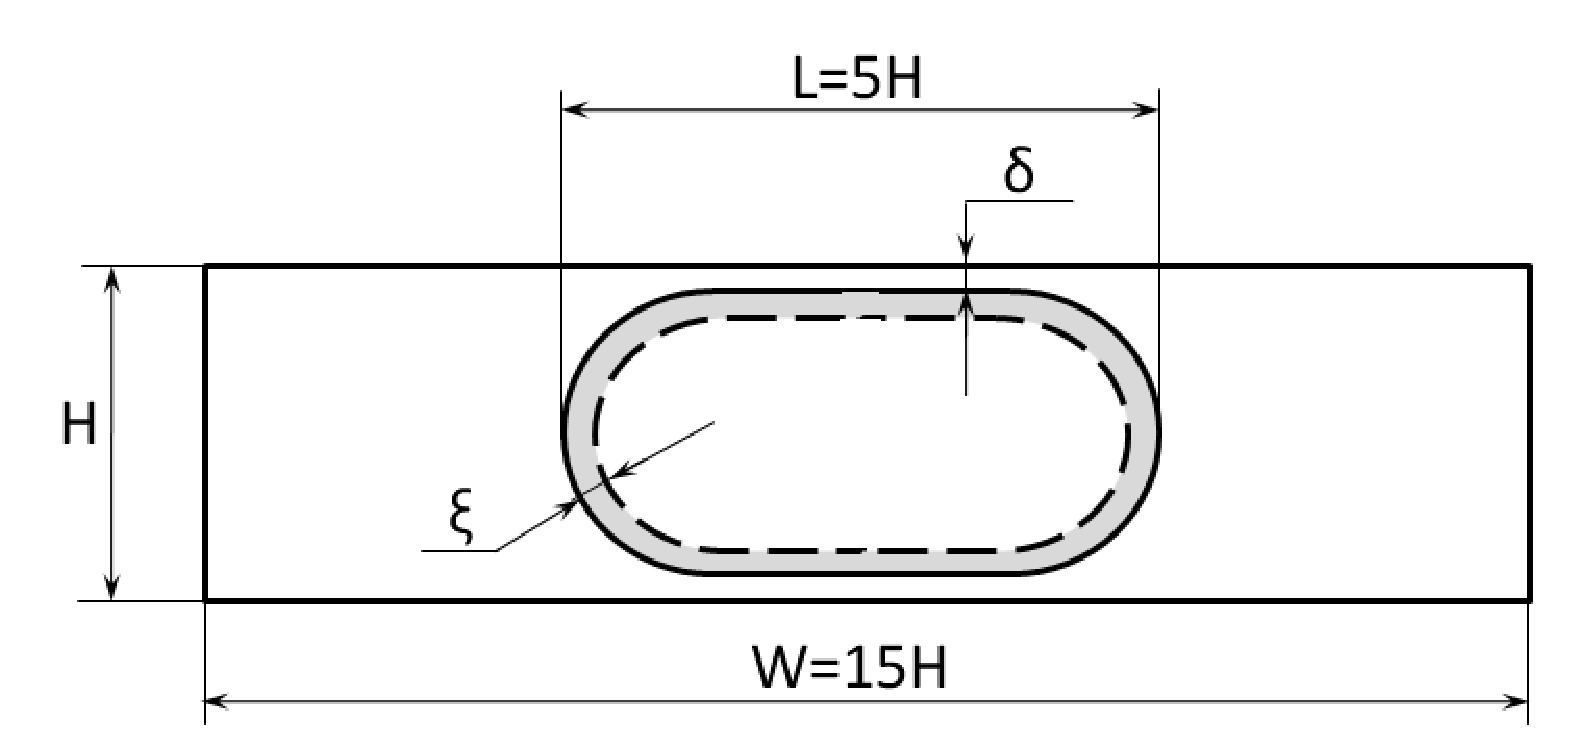
\includegraphics[width=0.97\textwidth]{Figures/benchmark.eps}
\caption{The benchmark sketch. $\delta$ corresponds to film thickness. $\xi$ corresponds to the interface thickness. We take the microchannel length to be 15 times larger than its height.
\label{fig:benchmark:sketch}}
\end{figure}


\section{Results}
\subsection{The nondimensionalization and initialization procedure}
We now introduce the procedure of nondimensionalization, as well as
the initialization technique we used to determine the parameters necessary for
the simulation. The capillary number defined in Eq.~\ref{capillary:number:definition} governs the interface thickness and is.
The bubble velocity $U_{\mathrm{bubble}}$ is taken in the center of the bubble where the film
thickness is examined.
While parameters such as $\mu_{\mathrm{liq}}$, $\gamma$ and the capillary number $\Ca$ are given
or defined through the model parameters, the bubble velocity $U_{\mathrm{bubble}}$ is not given
explicitly.
In our simulations we approximately match and initialize the velocity with the
Poiseuille profile center velocity, which is given as:
\begin{equation}
\begin{aligned}
U_{\mathrm{bubble}} \approx U_{\mathrm{liq}}=\frac{H_{\mathrm{eff}}^2}{8
\mu_{\mathrm{liq}}}\frac{\mathrm{d}P}{\mathrm{d}x}\\
U_{\mathrm{bubble}}\approx
\frac{{(N_y-2)}^2}{\frac{8}{6}(\tau_{\mathrm{liq}}-\frac{1}{2})}\frac{\mathrm{d}P}{\mathrm{d}
x } ,
\end{aligned}
\end{equation}
where $N_y$ is the grid number in the vertical direction. As will be discussed further, the
effective channel width is defined as $H_{\mathrm{eff}}=N_y-2$ because of bounce-back nodes.
For the Poiseuille profile one can estimate the body force (pressure gradient) through the
capillary number and grid resolution:
\begin{equation}
\label{poiseuille:velocity:center}
\begin{aligned}
&\frac{\mathrm{d}P}{\mathrm{d}x}=\frac{8}{{(N_y-2)}^2}\gamma \Ca.
\end{aligned}
\end{equation}
The body force (\ref{poiseuille:velocity:center}) causes the bubble
velocity to differ from that implied by the capillary number because of the bubble presence in a flow. That is
why the iteration proceduer is needed to achieve the 
desired velocity and 
capillary number. 
However, the initialization body force given by (\ref{poiseuille:velocity:center}) is a good
starting approximation. 

After one calculates the parameters necessary to run a simulation, one has to
initialize the macroscopic fields and particle populations.
The velocity is initialized with zero everywhere. Populations are initialized
using the equilibrium values for the binary liquid model, including all the phase
gradients and Laplacians. The liquid phase is initialized with $\phi = 1$ and the
gas phase with $\phi = -1$. Though the initial film thickness
does not affect the final result for the front meniscus (see Fig.
\ref{fig:different:initialization:widths}) we keep the initialized film
thickness as close as possible to the already obtained numerical film
thickness values \cite{giavedoni-numerical}. This is done to minimize
the time required for the simulation to be convergent, as starting far away from the steady-state requires
additional time for the relaxation.
\begin{figure}
\includegraphics*[bb=-15 360 630 430,width=0.97\textwidth]
{Figures/Init/initbegin12.eps}
\includegraphics*[bb=-15 360 630
430,width=0.97\textwidth]{Figures/Init/initfinish12.eps}\\
\includegraphics*[bb=-15 360 630 430,
width=0.97\textwidth]{Figures/Init/initbegin16.eps}
\includegraphics*[bb=-15 360 630
430,width=0.97\textwidth]{Figures/Init/initfinish16.eps}\\
\includegraphics*[bb=-15 360 630 430,
width=0.97\textwidth]{Figures/Init/initbegin20.eps}
\includegraphics*[bb=-15 360 630
430,width=0.97\textwidth]{Figures/Init/initfinish20.eps}\\
\caption{The phase plots for different bubble thicknesses as
$H_{\mathrm{eff}}-12$, $H_{\mathrm{eff}}-16$ and
$H_{\mathrm{eff}}-20$. The grid for the simulation is $102 \times 1501$. The results are rescaled
on $N_y$.The phase
profiles were obtained after $2\cdot10^5$ time steps. One can see that even if the
system is initialized with different bubble volumes, the bubbles always relax
to a shape where the film thickness is conserved. For the given parameters the
interface thickness rescaled at the effective channel width $H_{\mathrm{eff}}$  is
$0.0701$,$0.0697$,$0.0692$ measured at the dimensionless coordinate $x=13$.
\label{fig:different:initialization:widths}}
\end{figure}

Here, two different examples are presented that quantitatively show the
initialization procedure for different capillary numbers. In these
examples we use $k=0.04$ and $A=0.04$ as optimal binary liquid model parameters.
That explicitly implies the surface tension to be $\sqrt{\frac{8 k
A}{9}}=0.0377$ and the characteristic length of the interface
$5\sqrt{\frac{k}{A}}=5$ lattice Boltzmann units. For the sake of simplicity and
stability, the relaxation times for liquid and gas phases are taken as
$\tau_{\mathrm{liq}}=2.5$ and $\tau_{\mathrm{gas}}=0.7$, which correspond
to the gas liquid kinematic viscosity ratio equal to $10$.
\begin{description}
 \item[I \bm{$Ca=0.005$}]
  The film thickness for such small capillary numbers \cite{bretherton} is
given by the equation:
  \begin{equation}
  \frac{h_{\infty}}{H_{\mathrm{eff}}}=0.6687 \Ca^{2/3}=0.0194.
  \end{equation}
Thus, the film
 occupies about $2$ percent of the whole channel height. Let us impose that $8$ lattice
units are required to resolve  $2$ percent of the channel. Note that $5$ out of $8$ these lattice
units
($62.5$ percent) are used to resolve the phase interface. Therefore the channel width is $400$
lattice units.

We take the bubble length equal to $5$ channel widths
  and the distance between bubbles as $2$ bubble lengths. This gives a
grid size of $400 \times 6000$. In terms of computer memory
requirements, the calculations with double precision accuracy demand:
\begin{equation}
\begin{aligned}
&2\text{ sets of populations } \times \,\, 8\,\, \text{bytes per population
} \times \,\, 9 \text{
populations}\\
&\times\,400\,\times\,6000\approx 345 \mathrm{MB}. 
\end{aligned}
\end{equation}
Even using this naive assumption that the interface thickness is $62.5$ percent  of the
film thickness, one can get the memory
requirement of $345 \mathrm{MB}$. 

After resolving the interface one can  calculate the
  velocity from the capillary number as:
  \begin{equation}
  U_{\mathrm{bubble}}=0.005 \frac{\gamma}{\mu_{\mathrm{slug}}}=0.005
\frac{0.0377}{0.6666}=2.82 \cdot10^{-4},
  \end{equation}
  where $\mu_{\mathrm{slug}}=1/3 (2.5-0.5)=0.6666$.
  This velocity implies the following pressure gradient calculated from the
  Poiseuille flow solution, Eq. \ref{poiseuille:velocity:center}: 
  \begin{equation}
  \begin{aligned}
  \frac{\mathrm{d}P}{\mathrm{d}x}=9.42 \cdot 10^{-9}.
  \end{aligned}
  \end{equation}
Note that the velocity is directly
involved in calculation of the physical time step (small velocities imply longer running
simulations):
\begin{equation}
\Delta t =\frac{U_{\mathrm{LBM}}}{U_{\mathrm{phys}}} \Delta x ,
\end{equation}
where, for example, the real velocities in the physical world can reach
approximately $1$ m/s and the real height up to $1$ mm. In this case one
can easily approximate the physical time step during one lattice Boltzmann iteration:
\begin{equation}
\Delta t = 7.05 \cdot 10^{-10} \,\mathrm{s}
\end{equation}
which is small. A typical simulation runs approximately
$100000-300000$ time steps due to computational restrictions. That gives 
physical time simulation around $10^{-5}-10^{-4}\,\mathrm{s}$, which is
probably not enough for the physical system to come to the pseudo-steady state.

 \item[II $\bm{Ca=0.05}$] 
   The parameters in the previous subsection imply that long
computations are required in order for the system to come to equilibrium. The simulation becomes longer with a decrease of the
capillary number. Bretherton obtained an analytical solution for the range of low capillary
numbers $Ca \leq 0.005$. However, many researchers extended it to the range of capillary numbers
greater than
$0.005$, and to higher Reynolds numbers. One can refer to figures
  \ref{fig:giavedoni:planar} and \ref{fig:heil:planar} taken from the work of
  \citet{giavedoni-numerical,heil-bretherton}, who cross validated their
  simulations against the Bretherton data and each other. Even though the LBM can simulate
flows with small capillary numbers, i.e. less than $0.005$, the simulation time
is relatively long. Therefore, in our work we focus on the range of capillary numbers $\Ca$
employed by the simulations of
\citet{giavedoni-numerical} who cross validated
results for all ranges of capillary numbers.  Our intention is
  to show physically justified behavior for moderate parameters,
which
  can be easily and quickly validated on a computer.
  One can see from Fig.~\ref{fig:heil:planar} that the film thickness for the
  capillary number $0.05$ ranges from $0.12$ to $0.15$, while the Reynolds
  number from $0$ to $300$.

  The film thickness for such small capillary numbers is taken from Fig.~\ref{fig:heil:planar},
  and for Reynolds number $40$ equals $0.12$. We want to
  resolve $6\%$ of whole channel width with $12$ lattice units, where $5$
lattice units are related to the interface resolution.  Therefore, the channel
  width is $200$ lattice units and the grid size is $200 \times 3000$. The velocity can be
calculated from the capillary number as:
  \begin{equation}
  U_{\mathrm{bubble}}=0.05 \frac{\gamma}{\mu_{\mathrm{liq}}}=0.05 \frac{0.037712}{0.6666}=2.82\cdot
  10^{-3}.
  \end{equation}
  The velocity implies the following pressure gradient calculated from the
  Poiseuille flow solution:
  \begin{equation}
  \begin{aligned}
  &\frac{\mathrm{d}P}{\mathrm{d}x}=\frac{8}{N_y^2}\gamma \Ca=3.77\cdot10^{-7}.
  \end{aligned}
  \end{equation}
  Our approach to the initial conditions is  to take the flow parameters from the previously
performed
numerical simulations and to calculate the grid size from them, matching the
body force gradient through the solution for Poiseuille flow.

\end{description}
\begin{figure}
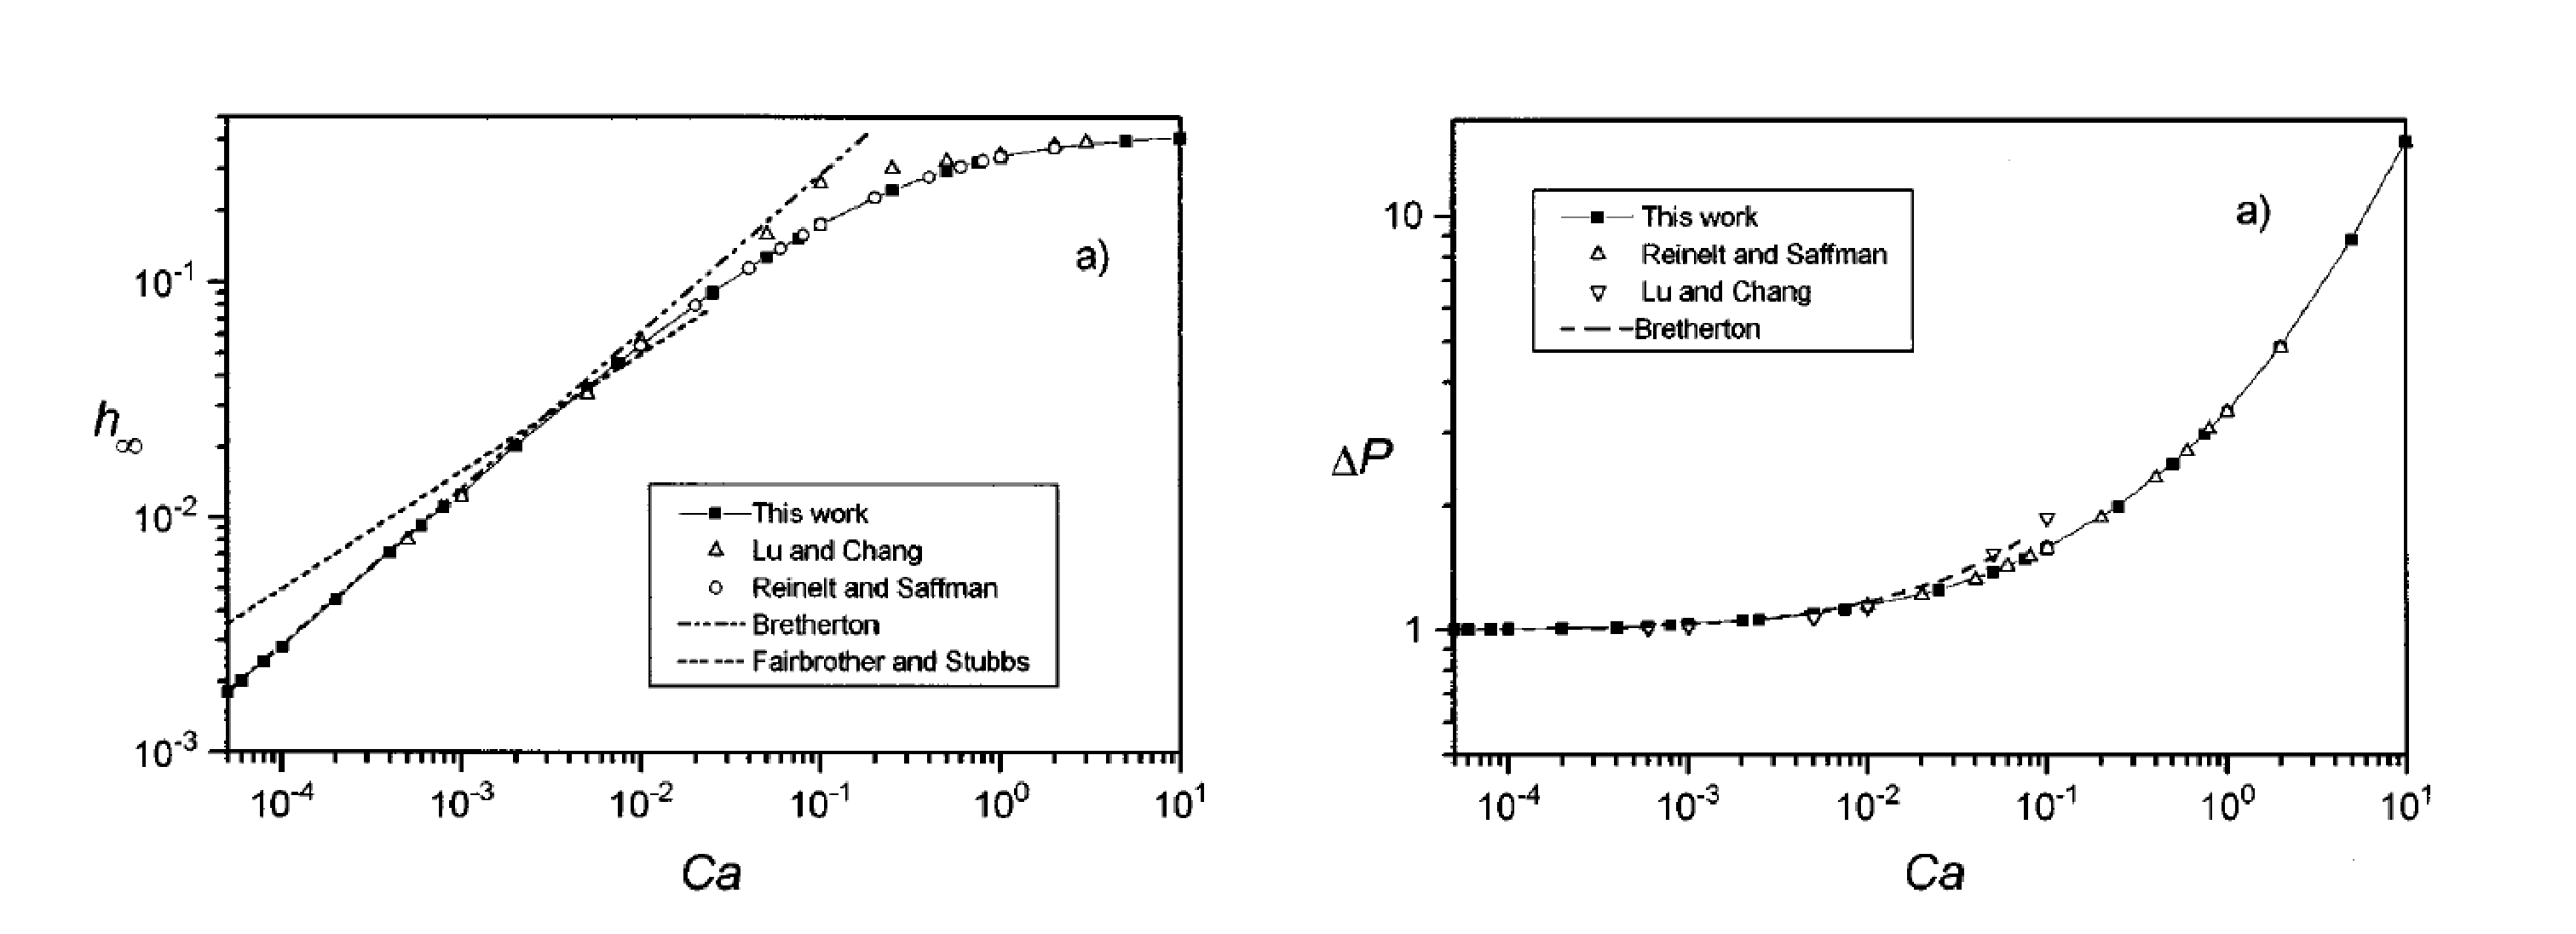
\includegraphics[width=0.97\textwidth]{Figures/giavedoni_planar.eps}
\caption{\citet{giavedoni-numerical} gathered results across the
literature for different capillary numbers. Note that results are scaled to the half-width of the
channel. \label{fig:giavedoni:planar}}
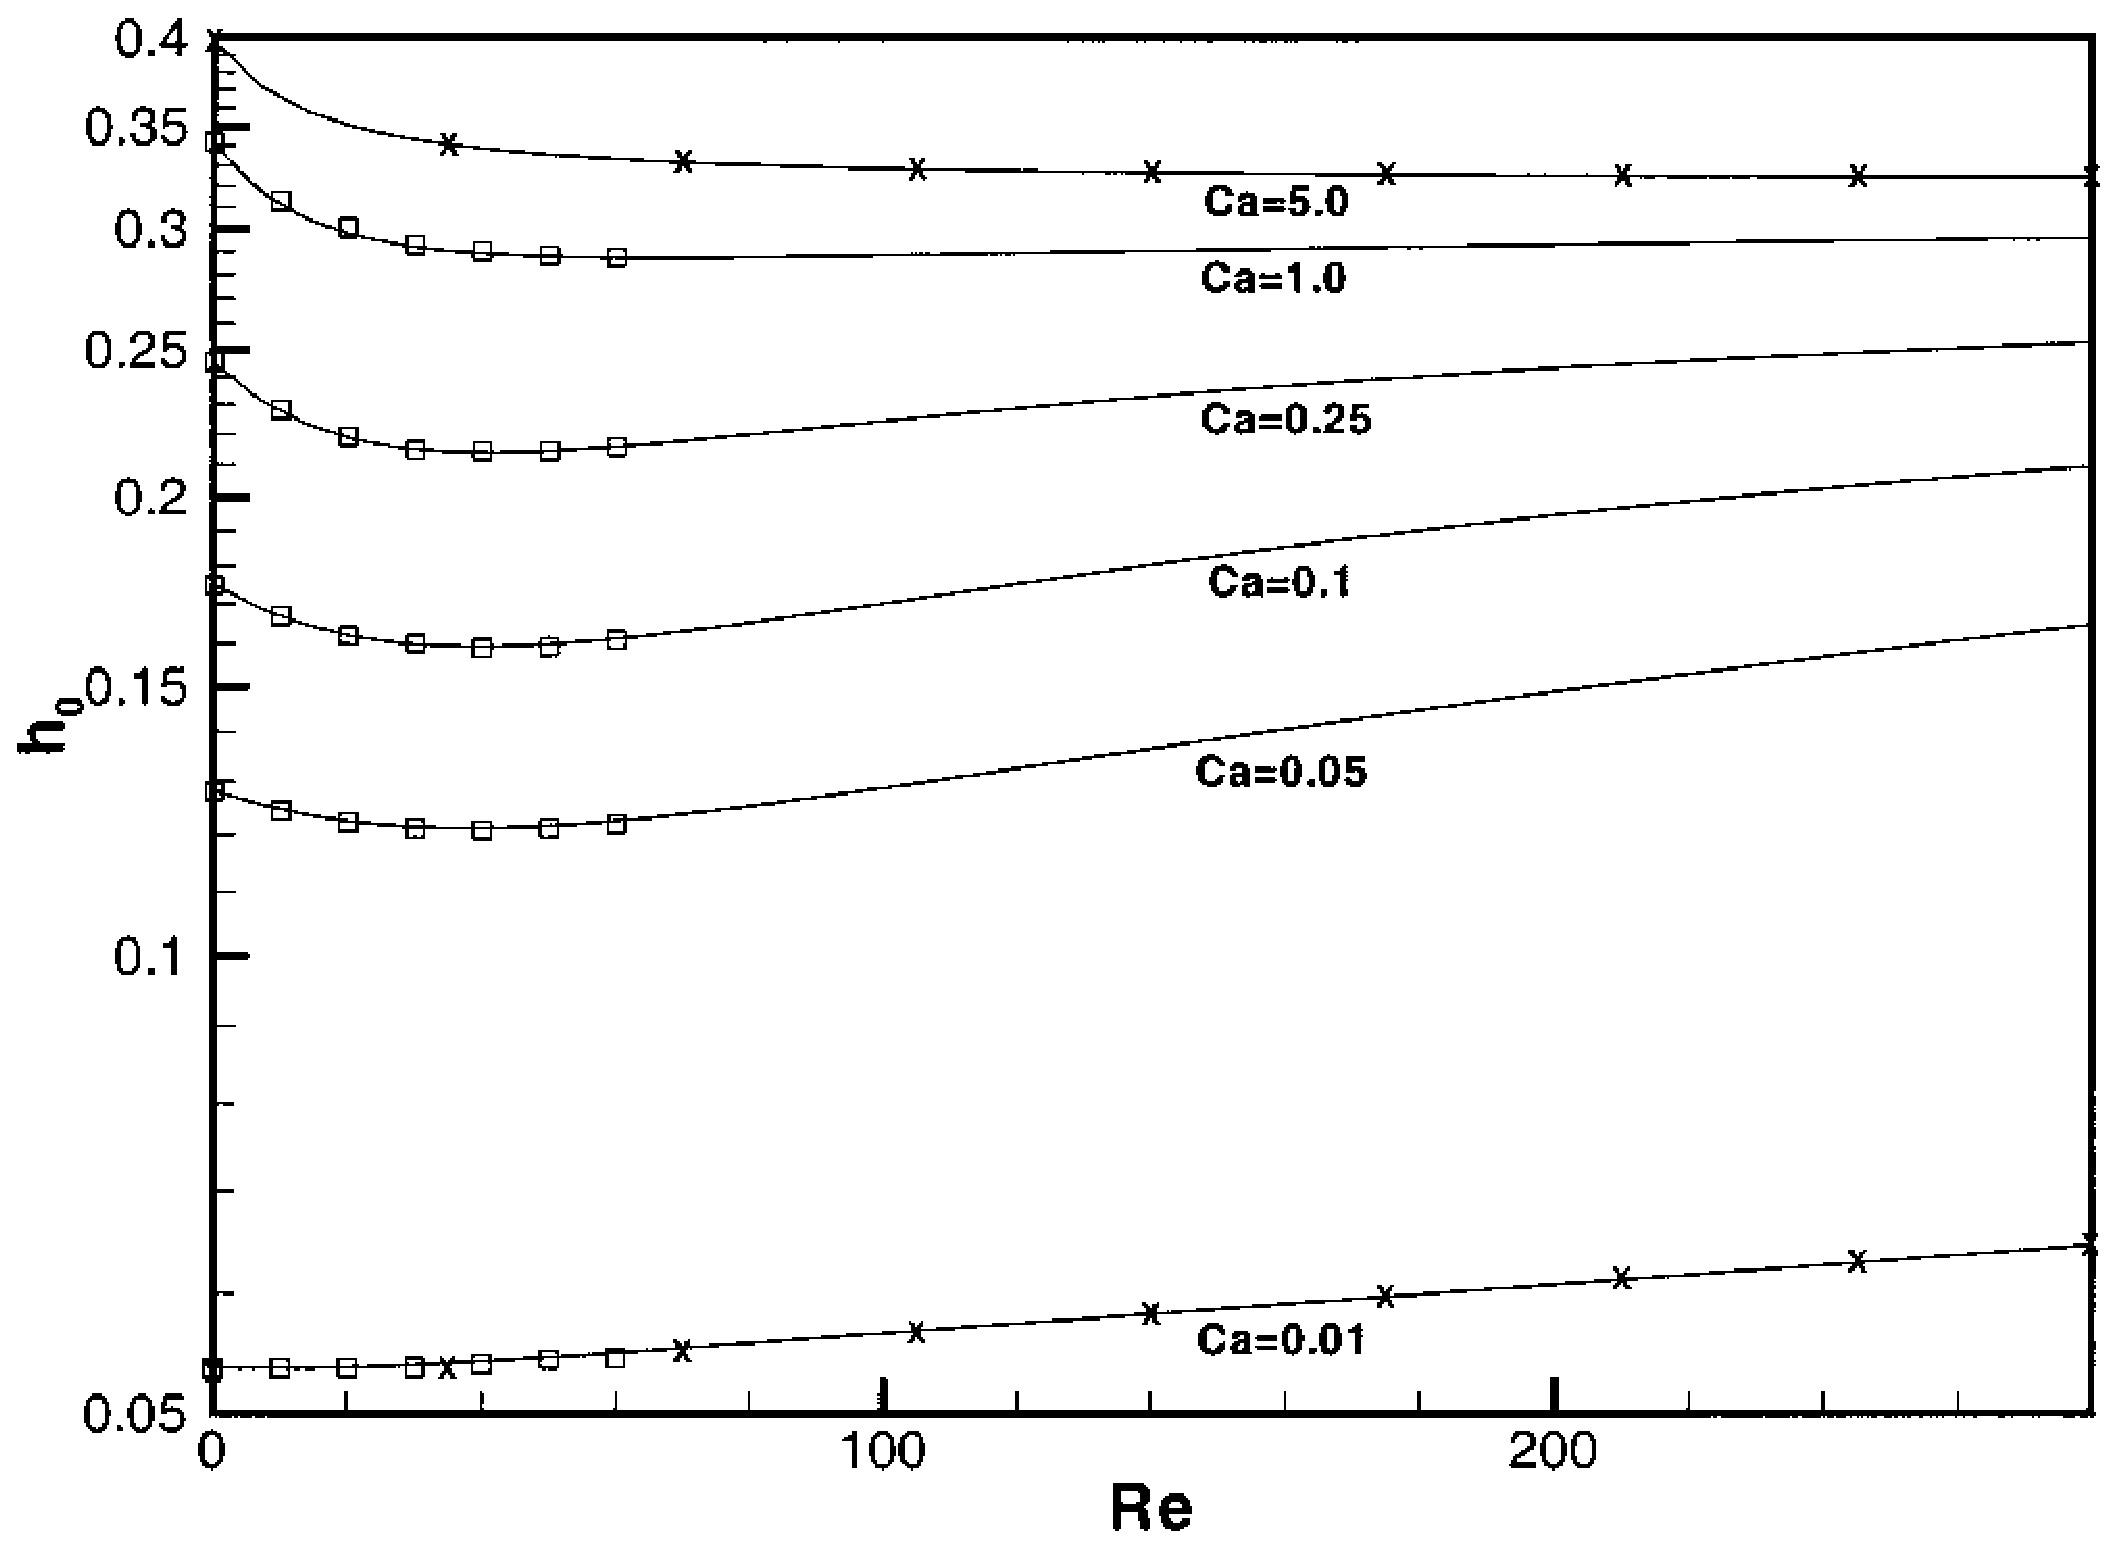
\includegraphics[width=0.97\textwidth]{Figures/heil-planar.eps}
\caption{\citet{heil-bretherton} performed simulations for different ranges of
capillary numbers and Reynolds numbers. Note that results are scaled to the half-width of the channel.
\label{fig:heil:planar}}
\end{figure}
Note that we base the initialization techniques on correlations for the
capillary number and the body force. However, in the binary liquid framework
those correlations are approximations. The strongest assumption is
in calculating the body force from the Poiseuille velocity profile.
In reality, the less viscous bubble moves faster than the surrounding liquid. By
substituting the obtained velocity in the capillary number equation, a
larger capillary number can be obtained. In practice, one needs to take the bubble velocity from the
simulations and
recalculate all the necessary flow characteristics, i.e. adjust the
 applied force to obtain the desired velocity/capillary number.

\subsection{Grid refinement}
To properly estimate the interface resolution one needs to study the convergence as a function of
the grid resolution. To do that the grid resolution is varies while all remaining parameters,
including the bubble velocity and the capillary number, are fixed.  Our goal is to determine the 
ratio of the interface thickness to the 
film thickness at which results are no longer dependent on the grid resolution.

Let us illustrate the procedure for the capillary number
$0.05$. As it was pointed out above, the film thickness in that case is $6$ percent of the
effective
channel $H_{\mathrm{eff}}$.
Note that in the case of the half-way bounce-back walls \cite{yu} which are used in the
simulations one needs to calculate the film thickness as:
\begin{equation}
\delta=(\phi_0-0.5)/(N_y-2),
\end{equation}
where $\phi_0$ is the grid coordinate where phase field is $0$, $N_y-2$
is related to the effective channel height.
If the grid size in the vertical direction is $N_y$, then one has $N_y-1$ regions between the grid nodes which represent
the physical domain. The effective wall location is in the middle between bounce-back and fluid nodes giving
overall $N_y-2$ nodes representing the fluid. Note that it is a big
simplification to impose the boundary in the middle between the bounce-back
node and the fluid node. The location of the wall for simple hydrodynamic flows is
viscosity dependent \cite{ginzburg-multireflection}.  Note that the effective location of the
wall for the
multiphase models to the best authors' knowledge is not yet derived. In the case of $\delta=0.06$
the
initial grid size is $N_y=102$, which gives the horizontal grid size as $N_x=15(N_y-2)=1500$.
The bubble is initialized as a rectangular box with coordinates
$y=7\dots N_y-8$, $x=\frac{N_x}{3}\dots \frac{2 N_x}{3}$ and phase
$\phi_{\mathrm{bubble}}=-1$. All other nodes are initialized with the phase field
$\phi=1$. The force gradient can be estimated through the Poiseuille
profile formula, Eq.~\ref{poiseuille:velocity:center}, and it equals
$1.508 \cdot 10^{-6}$ lattice units.

After choosing the reference parameters, the grid refinement procedure
needs to keep the macroscopic parameters constant.  It is easy to check
that it yields the following quantity to
be independent of grid size
$H_{\mathrm{eff}}^2\frac{\mathrm{d}P}{\mathrm{d}x}=(N_y-2)^2\frac{\mathrm{d}P}{\mathrm{d}
x } = \mathrm{const}$. We performed a number of simulations for the prescribed grids. The
simulation results in terms of grid numbers $N_x$, $N_y$, the film thickness $\delta$, center bubble
velocity $U_{bubble}$ are summarized in Table \ref{table:parameters:grid:refinement}.
The unified scaled profiles are shown in Fig. \ref{fig:grid:profiles}. One can
see that results converge for $H_{\mathrm{eff}}\geq 175$, and that with proper
initialization techniques, large enough time and different wall
wettabilities, results are different only in the 3rd digit even for
underresolved film thicknesses. To calculate how well the interface is
resolved, the ratio of the interface thickness to the film thickness is calculated. The
interface itself occupies approximately $5 \xi$, where
$\xi=\sqrt{k/A}=1$. The ratio of the interface thickness to the film thickness
$5\xi/H_{\mathrm{film}}$
 is shown in Table \ref{table:parameters:grid:refinement}. Based on these results one can conclude that
 the interface needs to be resolved as $40-50$ percent of the
expected film thickness for simulations to be convergent. We further examine the
velocities in the center of the bubble to calculate the capillary number. One can see from Table
\ref{table:parameters:grid:refinement} that the bubble velocities are pretty consistent and the
calculated capillary number corresponding to these velocities is $0.07$, which is slightly
larger than the expected capillary number. The corresponding error can be
attributed to the Poiseuille profile body force initialization and the
 density and viscosity ratios, which are much larger in the
Bretherton problem.
\begin{figure}
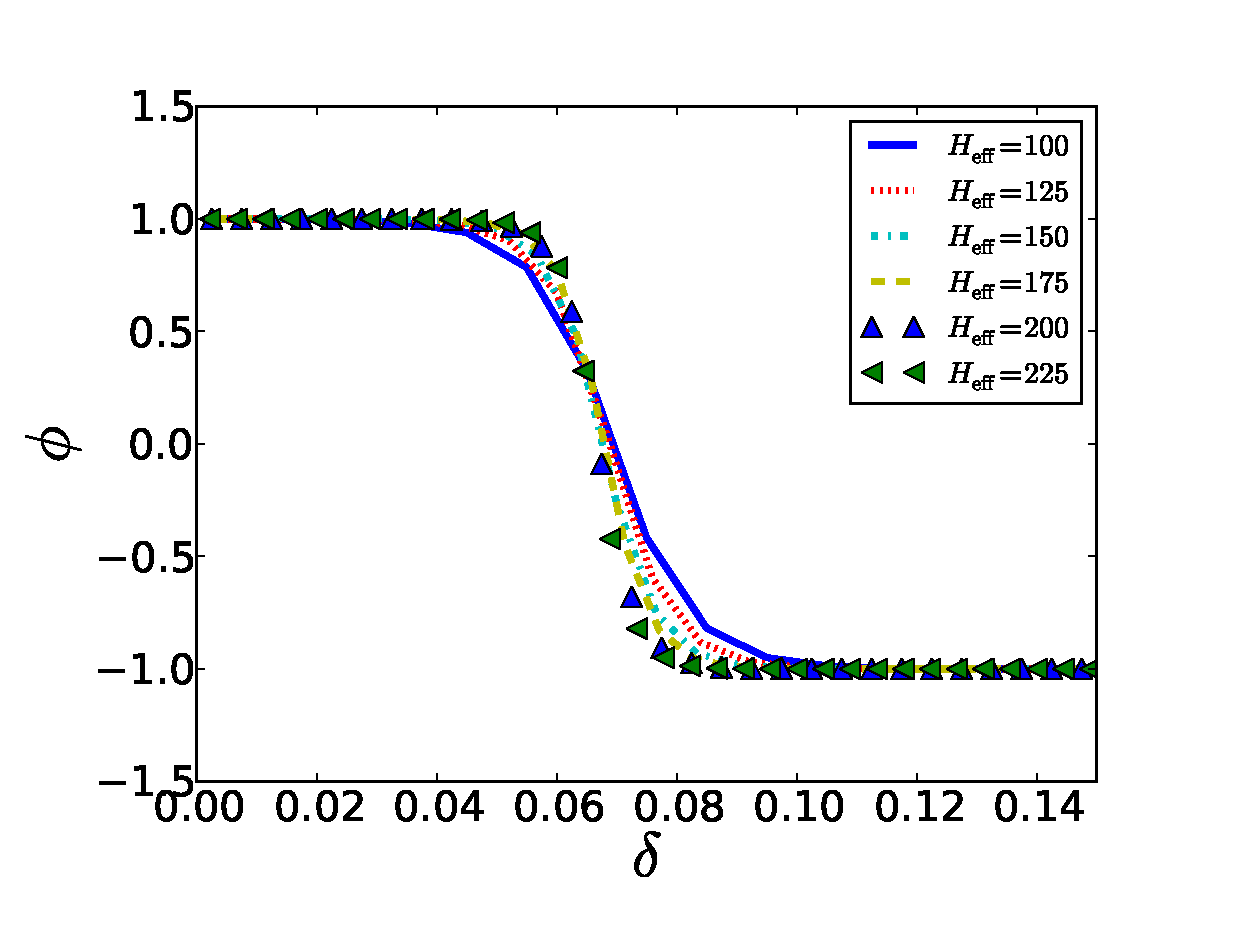
\includegraphics[width=0.97\textwidth]{Figures/Grid/norm_grid_profs.eps}
\caption{Grid-refined profiles for the effective
channel widths
$H_{\mathrm{eff}}=100,125,150,175,200,225$.$\delta$ is scaled on $H_\mathrm{eff}$ and $\delta=0$
corresponds to the wall location. The profiles were taken at $x=14$ (nondimensional coordinates).
Capillary number is $\Ca=0.05$. Capillary number obtained from simulations $\Ca=0.07$. One can
see
convergent results even for the underresolved film
thickness.\label{fig:grid:profiles}}
\end{figure}
%Here will be a consolidated table
\begin{table}
\begin{tabularx}{0.97\textwidth}{|X|X|X|X|X|X|}
\hline
$N_x$&$N_y$&$\delta$&$U_\mathrm{bubble}$&$\frac{5\xi}{H_{\mathrm{film}}}$&$N_\mathrm{iter}$\\
\hline
$1500$&$102$&$0.0694$&$0.0041$&$0.824$&$200000$\\
\hline
$1875$&$127$&$0.0688$&$0.0041$&$0.646$&$250000$\\
\hline
$2250$&$152$&$0.0676$&$0.0040$&$0.539$&$300000$\\
\hline
$2625$&$177$&$0.0679$&$0.0040$&$0.453$&$350000$\\
\hline
$3000$&$202$&$0.0668$&$0.0041$&$0.400$&$400000$\\
\hline
$3375$&$227$&$0.0663$&$0.0039$&$0.355$&$450000$\\
\hline
\end{tabularx}
\caption{The parameters and results for grid resolution simulations. Simulated domain is
of size $N_x \times N_y$. $U_\mathrm{bubble}$ is the velocity of the bubble center measured at
$x=14$.  $5\xi$ is the interface thickness. $H_{\mathrm{film}}=\delta (N_y-2)$ is the size of the film in
lattice Boltzmann units. $Ca=0.05$ was taken to initialize the simulation.
\label{table:parameters:grid:refinement}}
\end{table}

\subsection{The influence of the wall gradient}
The simulation results should not depend on the wall wettability. Wettability is defined
through the phase gradient \cite{pooley-contact}, $\partial_n \phi$.  We took a large
enough grid resolution in order for simulations to be consistent -- the grid size was
$177 \times 2626$ and the initial film thickness was
$12$ lattice Boltzmann units, which corresponds to the predicted film thickness.
We examined $11$ different values for the wall
gradient ranging from $-1$ to $1$. The parameters are summarized in Table
\ref{table:parameters:wall:gradient}. The results are consistent for all the
wall gradients given that the interface is properly resolved. For 
given wall gradients the values of interface thickness values are of $0.2\%$ relative accuracy.  For
the given wall gradients $0.8$
and $1.0$ the
simulations are unstable. One can see the calculated profiles in Fig.
\ref{fig:gradients:profiles}. The latter shows that the negative wall gradient values cause 
non-physical phase values (above $1.0$ near the wall). One should attribute them to the numerical
adjustment of wall gradients through a first-order finite difference scheme. Therefore, they do
not spoil numerical results. Note that
negative values of the phase gradient are
preferable, since the phase of the liquid adjacent to the wall has the value of $1$.
The phase values near the wall are above $1$ and do not interact
with the bubble which has phase value $-1$.  In case of positive
gradients the values near the wall are below $1$, and the gradient profile can
fuse with the values of the gas phase. This case corresponds to the slug flow when gas is in
contact with the wall.
\begin{figure}
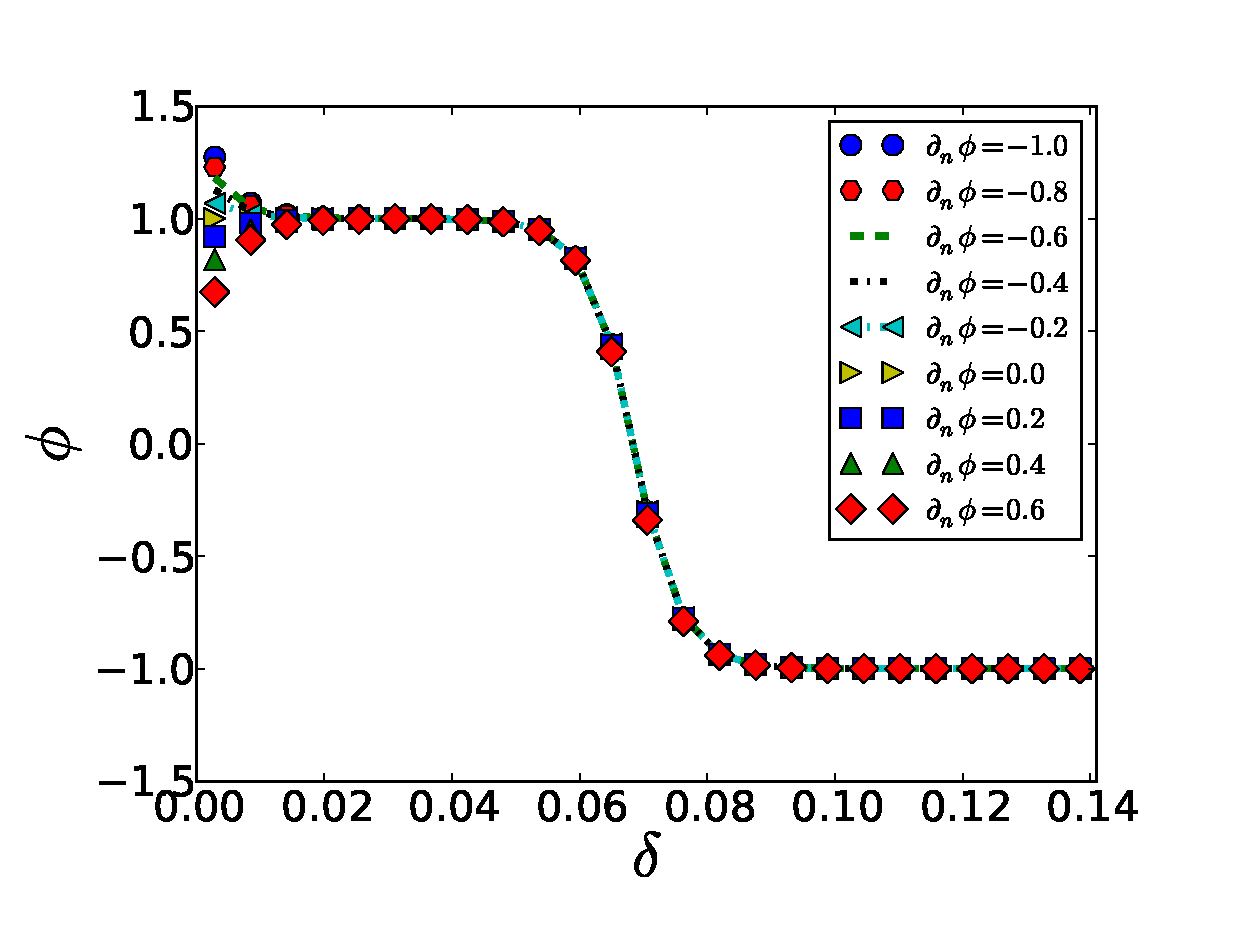
\includegraphics[width=0.97\textwidth]{Figures/Wall/phase_grad_profiles.eps}
\caption{Phase profiles for different wall gradients. One can see that if the thickness
is properly resolved then the wettability of the wall does affect the film thickness. The
simulations were conducted for $200,000$ iterations. The measured profile was taken at the
nondimensional coordinate scaled to $H_{\mathrm{eff}}$ as $x=11.42$. $\Ca=0.05$ was taken to
initialize simulation.
\label{fig:gradients:profiles}
}
\end{figure}

Another question that arises is the influence of the wall gradient on the bubble velocity and the
corresponding capillary number. The shear stress controlled by the wall phase gradient changes the
effective viscosity near the wall and the bubble velocity respectively. If the viscosity ratio is
high enough then the free surface motion of the bubble should not be dependent on the shear stress
near the wall.
One can see that if the film thickness is resolved properly the influence of the wall gradient can
be neglected. The velocities of the bubble center for certain profiles along $x$ direction are
presented in Table
\ref{table:parameters:wall:gradient}. 
%Fig. \ref{fig:velocities:wall:gradient} shows the center bubble velocity for different
%gradients. 
The average relative error for the mean velocity is $0.1\%$.
% Uncomment if you need this picture
% \begin{figure}
% 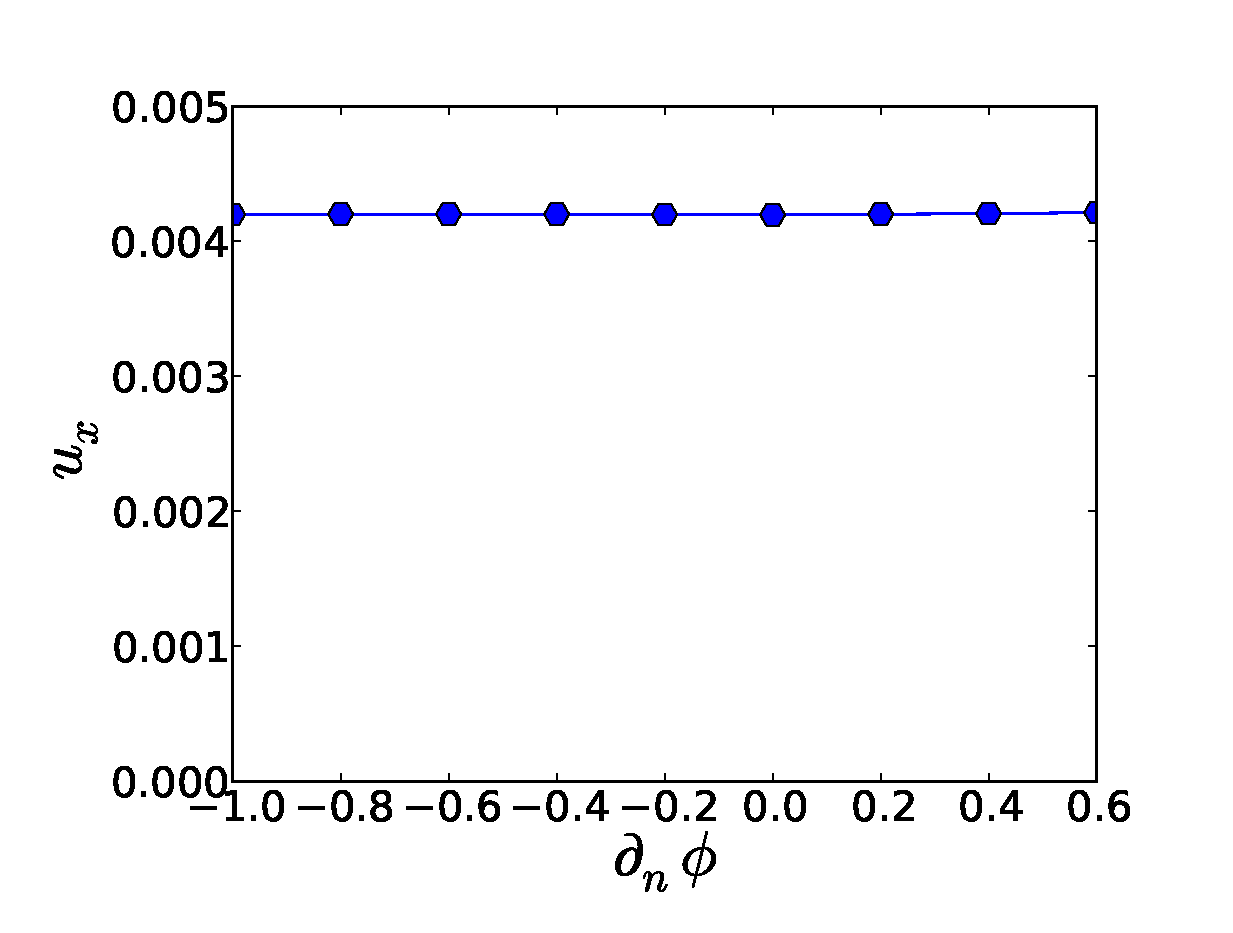
\includegraphics[width=0.97\textwidth]{Figures/Wall/velocities_grad_profiles.eps}
% \caption{The center bubble velocity versus the phase gradient. One can neglect the influence of
% the wall once the film is properly resolved.
% \label{fig:velocities:wall:gradient}
% }
% \end{figure}
\begin{table}
\begin{tabularx}{\textwidth}{|X|X X X X X X X X X X X|}
\hline
$\scriptstyle \partial_n \phi$& $\scriptstyle -1.0$& $\scriptstyle -0.8$&
$\scriptstyle -0.6$&$\scriptstyle -0.4$&$\scriptstyle -0.2$&$\scriptstyle
0.0$&$\scriptstyle 0.2$&$\scriptstyle 0.4$&$\scriptstyle 0.6$&$\scriptstyle 0.8$&$\scriptstyle
1.0$\\
\hline
$\scriptstyle \delta$& $\scriptstyle 0.0633$& $\scriptstyle 0.0634$& $\scriptstyle 0.0634$&
$\scriptstyle 0.0634$& $\scriptstyle 0.0634$& $\scriptstyle 0.0634$& $\scriptstyle 0.0633$&
$\scriptstyle 0.0632$& $\scriptstyle 0.0631$ &$\scriptstyle \mathrm{N/A}$&$\scriptstyle
\mathrm{N/A}$\\
\hline
$\scriptstyle U_{b}$ &$\scriptstyle 0.0041$& $\scriptstyle 0.0042$& $\scriptstyle 0.0042$
&$\scriptstyle 0.0042$ & $\scriptstyle 0.0041$& $\scriptstyle 0.0041$ & $\scriptstyle 0.0042$ &
$\scriptstyle 0.0042$ & $\scriptstyle 0.0042$ & $\scriptstyle \mathrm{N/A}$ &$\scriptstyle
\mathrm{N/A}$\\
\hline
\end{tabularx}
\caption{The parameters and results for wall gradient simulations. $U_{b}$ stands for the
center bubble velocity. $\delta$ is the interface thickness. $\partial_n \phi$ is the phase
gradient near the wall responsible for hydrophilic and hydrophobic behavior. The results are
calculated at nondimensional $x=11.42$ after $200 000$ time iterations. $\Ca=0.05$ was taken to
initialize simulation.
\label{table:parameters:wall:gradient}}
\end{table}

\subsection{Capillary number region}
The purpose of this section is to validate the correlations of
\citet{giavedoni-numerical}, Fig. \ref{fig:giavedoni:planar}, and
\citet{heil-bretherton}, Fig. \ref{fig:heil:planar}, for a range of capillary
numbers. Because of limited computational resources, we skip the
small capillary numbers and make calculations for the range of capillary numbers $0.03-0.8$, which
is a computationally reasonable task.  To be consistent with the previous sections, we choose the grid to be
$202 \times 3001$. $5$ lattice Boltzmann units do not occupy more than $60$
percent of the effective thickness. Because the simulation gets unstable with
smaller grids and larger gradients, all the capillary number simulations were
performed on the same grid. To properly initialize the force gradient, the
proportionality law was utilized. The forcing
$6 \cdot 10^{-6}/16$ was chosen to obtain the predicted capillary
number $0.05$. The forcing for other grids can be obtained using
simple proportionality relationships:
\begin{equation}
\begin{aligned}
&\Ca_{\mathrm{lit}} \propto U_{\mathrm{bubble}}\\
&U_{\mathrm{bubble}} \propto \frac{\mathrm{d}P}{\mathrm{d}x} N_y^2\\
&\Ca_{\mathrm{lit}} \propto \frac{\mathrm{d}P}{\mathrm{d} x} N_y^2 \text{ or }\\
&\frac{\mathrm{d}P}{\mathrm{d} x} \propto \frac{\Ca_{\mathrm{lit}}}{N_y^2},
\end{aligned}
\end{equation}
where the subscript ,,lit'' stands for the predicted capillary number
\cite{giavedoni-numerical,heil-bretherton}. The grid number $N_y$ is not
involved because all simulations are conducted on the same grid.
The pressure gradient can be obtained through the capillary number
ratio:
\begin{equation}
\frac{\mathrm{d}P}{\mathrm{d} x}=6 \cdot 10^{-6}/16 \frac{\Ca_{\mathrm{lit}}}{0.05}
\end{equation}
The film thickness is initialized through the ratio of capillary numbers as well:
\begin{equation*}
w=12 \frac{\Ca_{\mathrm{lit}}}{0.05}
\end{equation*}
The results obtained after $2\cdot10^5$ steps are presented in Table
\ref{table:parameters:capillary:number}. One can see that the calculated
capillary numbers are overpredicted but the obtained thicknesses are overpredicted
as well due to the improper body force setting caused by the Poiseuille flow assumption. If one
needs to obtain the desired capillary number, the shooting method for the forcing is
necessary, starting with the Poiseuille pressure gradient force as the initial condition. We extracted
the data of 
\citet{giavedoni-numerical} and \citet{heil-bretherton} and compared them with our results (see 
Fig. \ref{fig:capillary:comparison}).
\begin{figure}
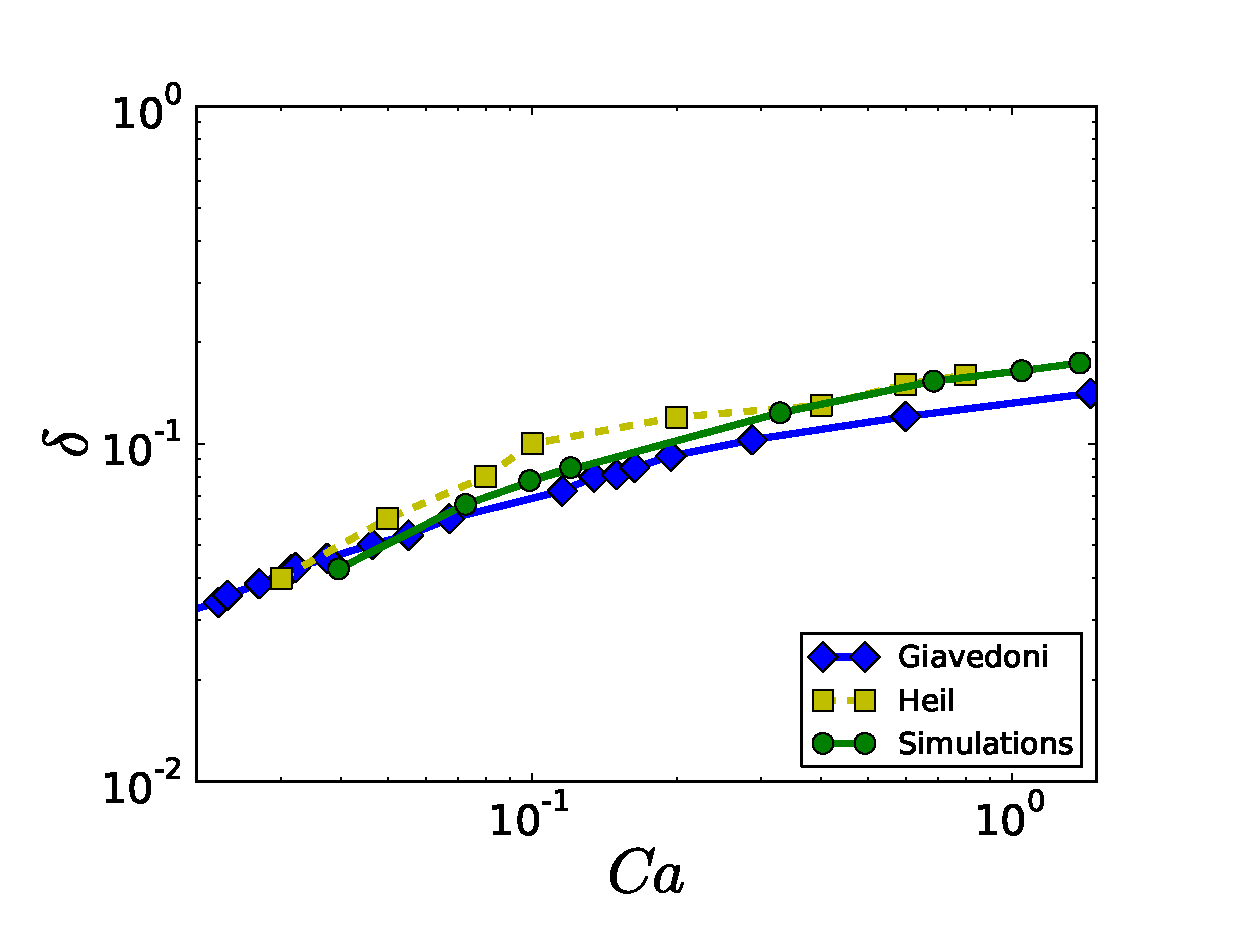
\includegraphics[width=0.97\textwidth]{Figures/Capillary/capillaries_comparison.eps}
\caption{A comparison between simulation results and results of
\citet{giavedoni-numerical} and \citet{heil-bretherton}. One can see a
reasonable agreement. The plots depict the film thickness as a function of the
the capillary number.\label{fig:capillary:comparison}}
\end{figure}

\begin{table}
\begin{tabularx}{\textwidth}{|X|X|X|X|X|X|}
\hline
$Ca_{\mathrm{lit}}$&$\delta_{\mathrm{lit}}$&$x$&$\delta$&$U_b$&$Ca$\\
\hline
$0.03$&$0.04$&$10.0$&$0.042$&$0.0022$&$0.039$\\
\hline
$0.05$&$0.06$&$11.0$&$0.066$&$0.0041$&$0.072$\\
\hline
$0.08$&$0.08$&$13.0$&$0.085$&$0.0068$&$0.120$\\
\hline
$0.1$&$0.1$&$12.5$&$0.077$&$0.0055$&$0.098$\\
\hline
$0.2$&$0.12$&$5.5$&$0.123$&$0.0185$&$0.328$\\
\hline
$0.4$&$0.13$&$4.7$&$0.153$&$0.0388$&$0.686$\\
\hline
$0.6$&$0.15$&$3.0$&$0.164$&$0.0592$&$1.046$\\
\hline
$0.8$&$0.16$&$1.7$&$0.173$&$0.0782$&$1.383$\\
\hline
\end{tabularx}
\caption{The parameters and results for capillary number region simulations.
$\delta_{\mathrm{lit}}$ is the film thickness with corresponding $\Ca_{\mathrm{lit}}$ taken from
literature. $\delta_\mathrm{sim}$ is the simulation film thickness with corresponding $\Ca$. $U_b$ is the
center bubble velocity taken at location $x$. $\Ca$ is based on the measured center bubble velocity
$U_{b}$.
\label{table:parameters:capillary:number}}
\end{table}



\subsection{The film variation over the bubble}

Next, we investigated the qualitative variation of the film thickness over the bubble length.
The comparison for the thickness variation is presented in Fig.~\ref{fig:sehgal:bubble:length}.
\begin{figure}
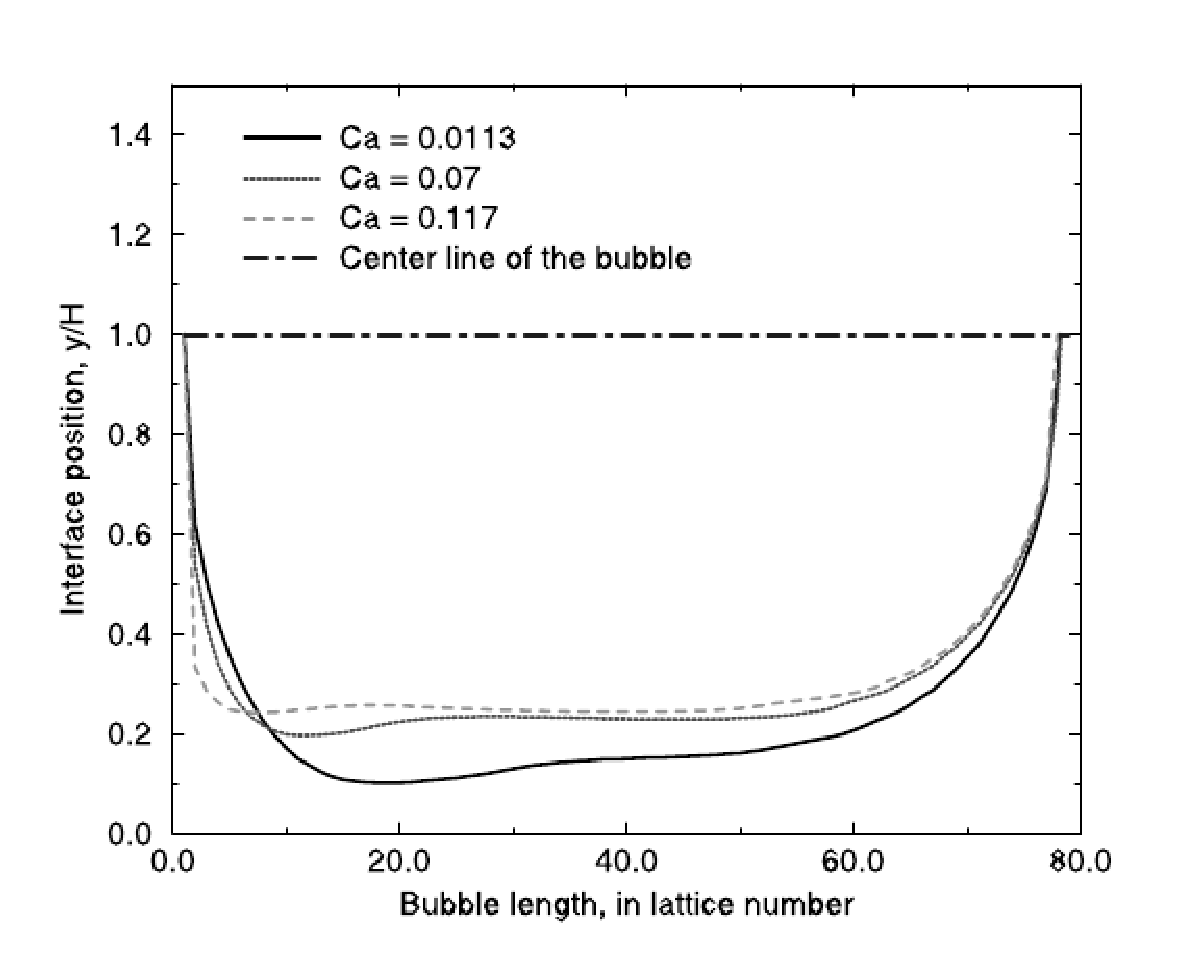
\includegraphics[width=0.47\textwidth]{Figures/Bubble/bubble_sehgal.eps}\hfill
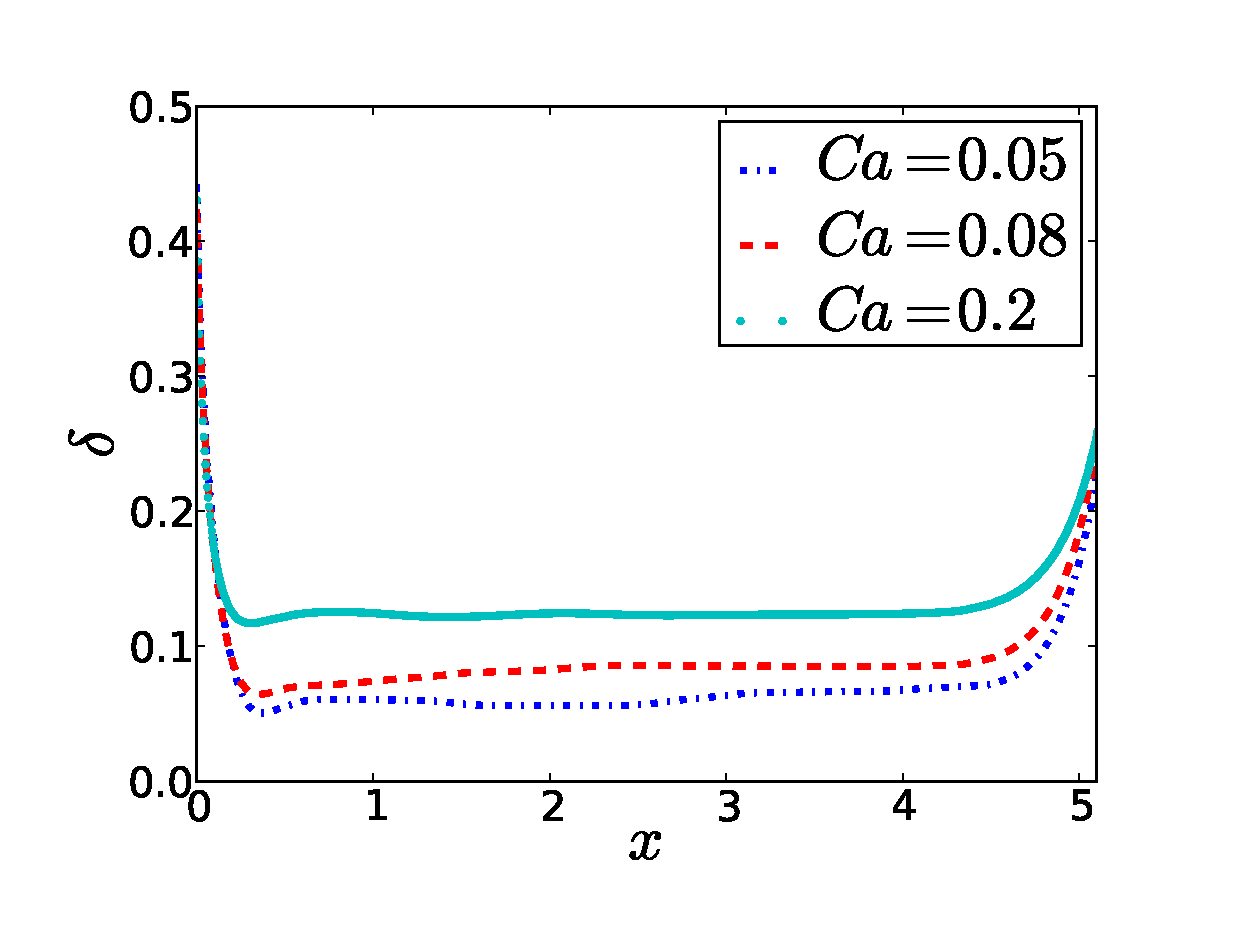
\includegraphics[width=0.47\textwidth]{Figures/Bubble/bubble_length.eps}\\
\caption{The qualitative comparison for the film thickness across
the bubble length. Left (courtesy of \citet{sehgal-microchannel}),
right (present simulations); $x$ is scaled to $H_{\mathrm{eff}}$
and increases in the flow direction.\label{fig:sehgal:bubble:length}}
\end{figure}
One can see a qualitative agreement, i.e. the thickness increases towards the front meniscus and
rapidly decreases towards the rear meniscus. This shape is sometimes referred to as a "bullet" shape.

\subsection{The influence of different viscosities}
The results presented above are taken for the liquid viscosity ratio $10$.
We performed the same simulations for the liquid-gas viscosity ratio of $20$.
The relaxation parameters were taken as $\tau_{\mathrm{liquid}}=4.5$ and $\tau_{\mathrm{bubble}}=0.7$. We
did not find any significant differences from the results presented above. The
comparison for the liquid film thicknesses is presented in Fig.
\ref{fig:capillary:viscous}. The results validate our assumption that in
the low capillary flow regime the density ratio does not affect the film thickness,
and that the gas-liquid viscosity ratio of the order $10$ is sufficient to obtain results
consistent with the literature data.
\begin{figure}
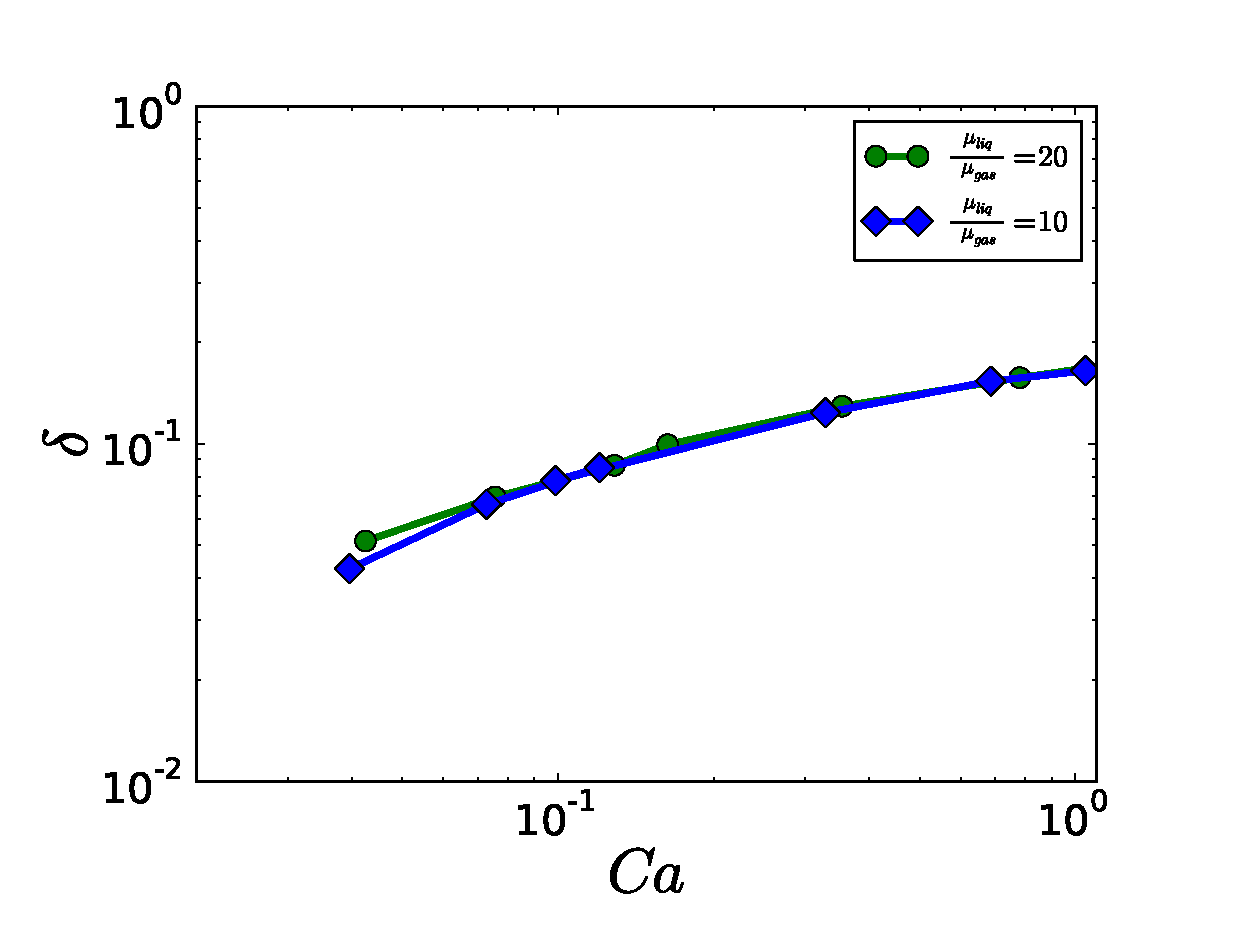
\includegraphics[width=0.97\textwidth]{Figures/Capillary_Viscous/capillaries_viscous.eps}
\caption{The film thicknesses versus capillary number for
$\frac{\mu_{\mathrm{liq}}}{\mu_{\mathrm{gas}}}=10$ and $\frac{\mu_{\mathrm{liq}}}{\mu_{\mathrm{gas}}}=20$. The
results show good consistency and mutual agreement.\label{fig:capillary:viscous}}
\end{figure}

\section{Conclusion}
This work presents numerical tips and a benchmark for the
Bretherton/Taylor problem using the binary liquid lattice Boltzmann method. The bubble was chosen sufficiently long for the film
thickness to
stabilize, and periodic boundary conditions were used to keep the simulations robust.  A bubble
train was simulated instead of the motion of a single bubble, and care was taken to minimize
the mutual influence of neighboring bubbles. The computational
results in terms of capillary number dependence and shape of the bubbles show consistency with the
previously published data. Surprisingly, with large enough viscosity ratio the results are
independent of any inertial effects.  An examination of the influence of grid resolution on the results allowed
us to determine that the phase interface should be resolved as at least $50$ percent of the simulated film thickness
in order for the simulations to be convergent. Though our results are specific to the binary liquid lattice
Boltzmann method, the numerical hints and procedures can be used for any
continuous interface method.
\bibliographystyle{model1-num-names}
\bibliography{paper}
%\bibliographystyle{unsrtnat}
%\bibliography{paper}
\end{document}
